%%%%%%%%%%%%%%%%%%%%%%%%%%%%%%%%%%%%%%%%%%%%%%%%%%%%%%%%%%%%%%%%%%%%%%%%%%%%%%%%%%%%%%%%%%%%%%%%%%%%%%%%%%%%%%%%%%%%%%%%%%%%%%%%%%%%%%%%%%%%%%%%%%%%%%%%%%%
% This is just an example/guide for you to refer to when submitting manuscripts to Frontiers, it is not mandatory to use Frontiers .cls files nor frontiers.tex  %
% This will only generate the Manuscript, the final article will be typeset by Frontiers after acceptance.   
%                                              %
%                                                                                                                                                         %
% When submitting your files, remember to upload this *tex file, the pdf generated with it, the *bib file (if bibliography is not within the *tex) and all the figures.
%%%%%%%%%%%%%%%%%%%%%%%%%%%%%%%%%%%%%%%%%%%%%%%%%%%%%%%%%%%%%%%%%%%%%%%%%%%%%%%%%%%%%%%%%%%%%%%%%%%%%%%%%%%%%%%%%%%%%%%%%%%%%%%%%%%%%%%%%%%%%%%%%%%%%%%%%%%

%%% Version 3.4 Generated 2018/06/15 %%%
%%% You will need to have the following packages installed: datetime, fmtcount, etoolbox, fcprefix, which are normally inlcuded in WinEdt. %%%
%%% In http://www.ctan.org/ you can find the packages and how to install them, if necessary. %%%
%%%  NB logo1.jpg is required in the path in order to correctly compile front page header %%%

\documentclass[utf8]{frontiersSCNS} % for Science, Engineering and Humanities and Social Sciences articles
%\documentclass[utf8]{frontiersHLTH} % for Health articles
%\documentclass[utf8]{frontiersFPHY} % for Physics and Applied Mathematics and Statistics articles

%\setcitestyle{square} % for Physics and Applied Mathematics and Statistics articles
\usepackage{url,hyperref,lineno,microtype,subcaption}
\usepackage[onehalfspacing]{setspace}

\linenumbers


% Leave a blank line between paragraphs instead of using \\


\def\keyFont{\fontsize{8}{11}\helveticabold }
\def\firstAuthorLast{Z. Cao {et~al.}} %use et al only if is more than 1 author
\def\Authors{Zhixuan Cao\,$^{1,2}$ Marcus Bursik\,$^{3}$  Qingyuan Yang\,$^{4,5}$ Abani Patra\,$^{\star,1,6}$}
% Affiliations should be keyed to the author's name with superscript numbers and be listed as follows: Laboratory, Institute, Department, Organization, City, State abbreviation (USA, Canada, Australia), and Country (without detailed address information such as city zip codes or street names).
% If one of the authors has a change of address, list the new address below the correspondence details using a superscript symbol and use the same symbol to indicate the author in the author list.
\def\Address{$^{1}$ Mechanical and Aerospace Engineering Department, SUNY Buffalo, Buffalo, NY, USA\\
$^{2}$Fluids Business Unit, ANSYS Inc, Lebanon, NH, USA \\
$^{3}$Center for Geohazards Studies, SUNY Buffalo, Buffalo, NY, USA  \\
$^{4}$Earth Observatory of Singapore,  Singapore,  Singapore\\
$^{5}$The Asian School of the Environment,  Nanyang Technological University, Singapore,  Singapore\\
$^{6}$Data Intensive Studies Center,  Tufts University, Medford, MA, USA}
% The Corresponding Author should be marked with an asterisk
% Provide the exact contact address (this time including street name and city zip code) and email of the corresponding author
\def\corrAuthor{Abani Patra}

\def\corrEmail{abani.patra@tufts.edu}

\begin{document}
\onecolumn
\firstpage{1}

\title[VATD Based on 3D Plume Model]{Simulating the transport and dispersal of volcanic ash clouds with initial conditions created by a 3D plume model} 

\author[\firstAuthorLast ]{\Authors} %This field will be automatically populated
\address{} %This field will be automatically populated
\correspondance{} %This field will be automatically populated

\extraAuth{}% If there are more than 1 corresponding author, comment this line and uncomment the next one.
%\extraAuth{corresponding Author2 \\ Laboratory X2, Institute X2, Department X2, Organization X2, Street X2, City X2 , State XX2 (only USA, Canada and Australia), Zip Code2, X2 Country X2, email2@uni2.edu}


\maketitle


\begin{abstract}

%%% Leave the Abstract empty if your article does not require one, please see the Summary Table for full details.
\section{}
 
Volcanic ash transport and dispersion (VATD) models simulate atmospheric transport of ash from a volcanic source represented by parametrized concentration of ash with height. Most VATD models use a source of some prescribed shape calibrated against an empirical expression for the height-mass eruption rate (MER) relation.
The actual vertical ash distribution in volcanic plumes usually varies from case to case and has complex dependencies on eruption source parameters and atmospheric conditions.
We present here for the first time the use of a three-dimensional (3D) plume model to represent the ash cloud source without any assumption regarding plume geometry. By eliminating assumed behavior associated with a parametrized plume geometry, the predictive skill of VATD simulations is greatly improved.
To date, no VATD simulation adopts initial conditions created from first principles based on a 3D plume simulation. We use our recently developed volcanic plume model based on a 3D smoothed-particle hydrodynamic Lagrangian method, and couple the output to a standard Lagrangian VATD model.  We apply the coupled model to the Pinatubo eruption in 1991 to illustrate the effectiveness of the approach.
Our investigation reveals that initial particle distribution in the vertical direction, including within the umbrella cloud, has more impact on transport of ash clouds than does the horizontal distribution. Comparison with satellite data indicates that ash particles are concentrated through the depth of the volcanic umbrella cloud, and much lower than the observed maximum plume height.

\tiny
 \keyFont{ \section{Keywords:}VATD, volcano, 3D plume model, initial conditions, numerical simulation, SPH, Pinatubo, ash transport, ash dispersal} %All article types: you may provide up to 8 keywords; at least 5 are mandatory.
\end{abstract}

\section{Introduction}
Volcanic ash, the fine-grained fraction of tephra, can be widely dispersed to synoptic and global scales, and can lead to a degradation of air quality and pose threats to aviation \citep{tupper2007facing}. Identification, tracking and modeling the future movement of volcanic ash help route and schedule flights to avoid ash clouds. Numerical estimation of ash distribution using known and forecast wind fields is necessary if we are to accurately predict ash cloud propagation and spread. Numerous volcanic ash transport and dispersion (VATD) models have been developed by both civil and military aviation, and meteorological agencies, to provide forecasts of ash cloud motion \citep{witham2007comparison}, such as Puff \citep{tanaka1991development,searcy1998puff}, NAME \citep{jones2007uk}, HYSPLIT \citep{stein2015noaa, rolph2017real} and Ash3d \citep{schwaiger2012ash3d}. New techniques have been integrated into VATDs to satisfy increasing demands for different types of output, model accuracy and forecast reliability. This contribution explores a forward modeling method for creating initial conditions for VATD simulations, which promises to reduce the need for inversion or user intervention and improve forecasting.

\citet{fero2009simulating} and \citet{stohl2011determination} showed that initial source conditions have significant effects on simulation of volcanic ash transport. \citet{constantinescu2021radius} proved that an enhanced initial condition provides an overall better fit of the tephra deposit generated from an ash cloud than do models without a disk-like source, demonstrating the significant impact of initial condition on ash dispersion. Besides  location of the eruption vent and timing of the release, traditional VATD simulation requires key global descriptors of the volcanic plume, especially plume height, grain size, eruption duration and mass loading, or alternatively, a mass eruption rate (MER). No matter how these global descriptors are obtained, they are used to furnish the initial conditions for VATDs in the form of a line-source term of a spatio-temporal distribution of particle mass. It is a common practice to pick values for these global descriptors using an empirical expression for the height-MER relation. The values for the descriptors can also be found by parameter calibration or inversion \citep[e.g.][]{fero2008simulation,fero2009simulating, stohl2011determination, zidikheri2017estimation}. One-dimensional (1D) plume models serve as an alternative option to provide these values. For example, \citet{bursik2012estimation} used the 1D model puffin \citep{bursik2001effect} to generate estimates of mass eruption rate and grain size. In some cases, an extra step is adopted to spread ash particles from the line source horizontally, resulting in an initial ash cloud in 3D space. The horizontal spreading depends on an empirical expression as well. For example, the VATD model Puff spreads particles from the line source uniformly in the horizontal direction within a given radius. Considering the complexities of volcanic eruptions, the actual ash distribution in the initial cloud should vary from case to case and with time, making it difficult to find one general expression that is suitable for all cases. It is useful therefore to investigate alternative ways for creating initial ash clouds without assumptions regarding plume geometry, or numerical inversion. This provides the major motivation of this paper.

VATD models can be categorized into Lagrangian particle tracking and
Eulerian advection-diffusion types. Among several available particle
tracking models, such as, Hypact \citep{walko1995hypact}, Puff
\citep{searcy1998puff}, CANERM \citep{d1998modeling}, and HYSPLIT
\citep{draxler1998overview} and advection-diffusion models, such as
Fall3D \citep{folch2009fall3d}, and Ash3D \citep{schwaiger2012ash3d},
we adopt a particle tracking model, Puff, as the primary VATD
model. Puff can accept a 3D point cloud description of the starting
ash cloud as an initial condition, which makes it technically easier
to couple with a 3D Lagrangian plume model. Puff initializes a
discrete number of tracers that represent a sample of the eruption
cloud, and calculates transport, turbulent dispersion, and fallout for
each representative tracer. A cylinder extending vertically from the
volcano summit to a specified plume height is the standard approach to
provide a simple model of the geometry of a typical ash column. Puff
minimally requires horizontal wind field data. The ``restart'' feature
of Puff makes it feasible to accommodate the hand-off between a plume
simulation and the Puff simulation in terms of time and length
scales. We use the Hybrid Single-Particle Lagrangian Integrated
Trajectory model (HYSPLIT) \citep{stein2015noaa, rolph2017real} to
better understand simulation results from Puff in this study.

Besides parameter calibration, 1D plume models have been used to obtain global descriptors of volcanic plumes. 1D plume models \citep [e.g.][]{woods1988fluid, bursik2001effect, mastin2007user, de2015plume, folch2016fplume, pouget2016sensitivity} solve the equations of motion in 1D using simplifying assumptions, and hence depend on estimation of certain parameters, especially those related to the entrainment of air, which is evaluated based on two coefficients: a coefficient due to turbulence in the rising buoyant jet, and one due to the crosswind field. Different 1D models adopt different entrainment coefficients based on a specific formulation or calibration against well-documented case studies. The feedback from plume to atmosphere is usually ignored in 1D models. While these 1D models generate well-matched results with 3D models for plumes that are dominated by wind (often called weak plumes) much greater variability is observed for strong plume scenarios \citep{bursik2009volcanic, costa2016results}. On the other hand, 3D numerical models for volcanic plumes based on first principles and having few parametrized coefficients \citep{oberhuber1998volcanic, neri2003multiparticle, suzuki2005numerical, cerminara2016ashee, cao2018plume} naturally create a 3D ash cloud, which could serve directly as an initial state of the volcanic material for VATDs. However, there is no VATD simulation using such 3D ash clouds as initial conditions. In this paper, we will carry out VATD simulations using an initial state for the ash cloud based on 3D plume simulations, generated with Plume-SPH \citep{cao2018plume, cao2017data}. The implementation techniques described in this paper can be applied to any combination of VATD model and 3D plume model even though our investigation is based on a specific VATD model and plume model.

The 1991 eruption of Pinatubo volcano is used as a case study. Pinatubo erupted between June 12 and 16, 1991, after weeks of precursory activity. The climactic phase started on June 15 at 0441 UTC and ended around 1341 UTC \citep{holasek1996satellite}. The climactic phase generated voluminous pyroclastic flows, and sent Plinian and co-ignimbrite ash and gas columns to great altitudes \citep{scott1996pyroclastic}. The evolution of the Pinatubo ash and \texorpdfstring{SO\textsubscript{2}} clouds was tracked using visible \citep{holasek1996satellite}, ultraviolet (Total Ozone Mapping Spectrometer; TOMS) \citep{guo2004re} and infrared sensors, including the Advanced Very High-Resolution Radiometer (AVHRR) \citep{guo2004particles}. There is sufficient observational data to estimate the eruption conditions for the climactic phase of the eruption \citep{suzuki2009three}. The availability of calibrated eruption conditions and extensive observational data regarding ash cloud transport make the Pinatubo eruption an ideal case study.

\section{Materials and Methods} \label{sec:Methodology}

\subsection {Plume-SPH Model} \label{sec:plume-sph}
Plume-SPH  \citep{cao2018plume} is designed to describe an injection of well mixed solid and volcanic gas from a circular vent above a flat surface into a stratified stationary atmosphere. The basic assumptions of the model are: 
\begin{enumerate}
\item Molecular viscosity and heat conduction is neglected since turbulent energy and momentum exchange are dominant.
\item Erupted material consisting of solid with different size and mixture of gases  is assumed to be well mixed and behave like a single phase fluid (phase 2) which is valid for eruptions with fine particles and ash.
\item Air, which is assumed to be a well mixed mixture of different gases, is assumed to be another phase (phase 1).
\item Assume thermodynamic equilibrium and dynamic equilibrium between the two phases. As a result, both phases share the common energy equation and momentum equations.
\item All other microphysical processes (such as the phase changes of \texorpdfstring{H\textsubscript{2}O}, aggregation, disaggregation, absorption of gas on the surface of solids, solution of gas into a liquid) and chemical processes are not considered in this model.
\item The effect of wind is also not currently considered in this model. 
\end{enumerate}

Based on above assumptions, the governing equations of our model are given as:
\begin{align}
\dfrac{\partial \rho}{\partial t} + \nabla \cdot \left(\rho \textbf{v}\right) = 0 \label{eq:gov-cs-rho} \\
\dfrac{\partial \rho \xi}{\partial t} + \nabla \cdot \left(\rho \xi \textbf{v}\right) = 0 \label{eq:gov-cs-ks}\\
\dfrac{\partial \rho \textbf{v}}{\partial t} + \nabla \cdot \left(\rho \textbf{v} \textbf{v} + p\textbf{I}\right) = \rho \textbf{g} \label{eq:gov-cs-v} \\
\dfrac{\partial \rho E}{\partial t} + \nabla \cdot \left[\left(\rho E + p \right)\textbf{v}\right] = \rho \textbf{g} \cdot\textbf{v} \label{eq:gov-cs-e}
\end{align}
where $\rho$ is the density, $\textbf{v}$ is the velocity, $\xi$ is the mass fraction of ejected material, $\textbf{g}$ is the gravitational acceleration, $\textbf{I}$ is a unit tensor.
$E = e + K $ is the total energy which is a summation of kinetic energy $K$ and internal energy $e$.
An additional equation is required to close the system. In this model, the equation for closing the system is the following equation of state (EOS).
\begin{equation}
p = \left(\gamma_m - 1\right)\rho e \label{eq:EOS}
\end{equation}
where
\begin{equation}
\gamma_m = R_m/C_{vm} + 1 \label{eq:gov-gm}
\end{equation}
\begin{equation}
R_m = \xi_g R_g + \xi_a R_a  \label{eq:gov-Rm}
\end{equation}
\begin{equation}
C_{vm} = \xi_s C_{vs} + \xi_g C_{vg} + \xi_a C_{va} \label{eq:gov-Cvm}
\end{equation}
\begin{equation}
\xi_a = 1 - \xi \label{eq:gov-na}
\end{equation}
\begin{equation}
\xi_g = \xi \cdot \xi_{g0} \label{eq:gov-ng}
\end{equation}
\begin{equation}
\xi_s = \xi - \xi_g \label{eq:gov-ns}
\end{equation}
where, $C_v$ is the specific heat with constant volume, $R$ is the gas constant. $\xi$ is the mass fraction of erupted material. The subscript $m$ represents mixture of ejected material and air, $s$ represents solid portion in the ejected material, $g$ represents gas portion in the ejected material, $a$ represents air, $0$ represents physical properties of erupted material. $\xi_{g0}$ is the mass fraction of vapor in the erupted material.

Three different boundary conditions are applied in this model. At the vent, temperature of erupted material $T$, eruption velocity $\textbf{v}$, the mass fraction of vapor in erupted material $\xi_{g0}$ and mass discharge rate $\dot M$ are given. The pressure of erupted material $p$ is assumed to be the same as ambient pressure for pressure-balanced eruption. The radius of the vent is determined from $\rho$, $\dot M$ and $\textbf{v}$.  Non-slip wall boundary condition is applied to the flat ground, where we enforce the velocity to be zero. With further assumption that the ground is adiabatic, internal energy flux, which consists of heat flux and energy flux carried by mass flux, vanishes on the wall boundary. Pressure outlet boundary condition is applied to the surrounding atmosphere where the pressure is given. Except for the pressure,  boundary values for density, velocity, and energy are determined by numerical calculation from the conservation laws. The initial condition for Plume-SPH is created based on the atmosphere profile before the eruption. 

The governing equations,  EOS, boundary conditions, and initial conditions establish a complete mathematical model. The model posed over the computational domain is then discretized using smoothed particle hydrodynamics (SPH) method \citep{gingold1977smoothed} available in the tool  Plume-SPH \citep{cao2017data, cao2018plume} using two types of SPH particles: 1) particles of phase 1 to represent ambient air, and 2) particles of phase 2 to represent erupted material. So before the eruption, the computational domain is fully occupied by particles of phase 1. During the eruption, particles of phase 2 are injected into the computational domain. The discretized model is then converted into a large computation  task in the Plume-SPH tool based on a parallel data management framework \citep{cao2017data}.

The input parameters for Plume-SPH include the eruption condition at vent, the material properties, and a profile of the atmosphere. The eruption parameters, material properties and atmosphere for the ``Strong plume--no wind'' case in the recent comparison study on eruptive column models \citep {costa2016results} are adopted. Eruption conditions and material properties are listed in Table \ref{tab:input_parameters_plume_simulation}. Note that the density of erupted material at the vent and radius of the vent can be computed from the given parameters. The eruption pressure is assumed to be the same as the atmospheric pressure at the vent, hence is not given in the table. The vertical profiles of atmospheric properties were  based on the reanalysis data from European Centre for Medium-Range Weather Forecasts (ECMWF) for the period corresponding to the climactic phase of the Pinatubo eruption. 

Running of Plume-SPH updates physical quantities, such as temperature, velocity, and the position of SPH particles in each time step. During Plume-SPH simulation, SPH particles of phase 2, which represent the erupted material, are injected from the eruption vent into the computation domain with an initial injection velocity. As they move upwards, these particles will get mixed with SPH particles of phase 1, which represent the air, during the whole simulation. Their physics quantities get updated as well. After the simulation, the computation domain will be filled with SPH particles of both phase 1 and phase 2. Removing all SPH particles of phase 1 from the computation domain, all of the remaining SPH particles  represent the erupted material, which naturally forms a plume (see  Fig. \ref{fig:create-initial-ash-plume-sph}). 

\subsection{Puff and Initial Ash Cloud} \label{sec:puff-model}
Puff \citep{tanaka1991development,searcy1998puff} is a dynamic pollutant tracer model. The model is based on a 3D Lagrangian form of the fluid mechanics, in which the material transport is represented by the fluid motion, and diffusion is parameterized by a stochastic process of random walk. Here, the model is constructed by a sufficiently large number of  Lagrangian tracer particles with a random variables $\textbf{R}_i(t) = (x(t),y(t),z(t))$, where $ i = \mbox{1} \sim M$, which represent position vectors of particles from the origin of the ash source at the time $t$. $M$ is the total number of  Lagrangian tracer particles, a sample of all the ash particles.
\begin{equation}
\textbf{R}_i(t+\Delta t) = \textbf{R}_i(t) + \textbf{W}(t)\Delta t + \textbf{Z}(t)\Delta t + \textbf{S}_i(t) \Delta t
\label{eq:puff-model}
\end{equation}

Here, $\textbf{W}$ accounts for local wind advection, $\textbf{Z}$  is generated by Gaussian random numbers and accounts for turbulent dispersion, and $\textbf{S}$ is the terminal gravitational fallout velocity or settling speed, which depends on a tracer's size.

A collection of tracer particles can be used to start a Puff simulation. The tracer particles have three basic properties, age, size and position. The age of each particle is the elapsed time from when it was released. Ash particles in the initial ash cloud have zero age. Initial ash size distribution is assumed to be log-normal. According to a mean and standard deviation provided by the user, Puff assigns size to each particle. Puff initializes the position of each particle according to semiempirical expressions. The height of each particle is determined according to the specified distribution from the surface (1000 mbar $\cong$ 0 m) to the top of the plume height, $H_{max}$, which is given by the user. Puff also supports reading predefined initial ash clouds from a file, containing the coordinates of all tracer particles. 

Vertical particle distribution in Puff is usually based on the Poisson distribution. For the Poisson distribution, the vertical height of ash particles is given by Eq. (\ref{eq:Poisson-plume-shape}):
\begin{equation}
H=H_{max} - 0.5 H_{width}P+H_{width}R
\label{eq:Poisson-plume-shape}
\end{equation}
where $P$ is an integral value drawn from a Poisson distribution of unit mean, $R$ is a uniformly distributed random number between 0 and 1, $H_{max}$ is the maximum plume height, $H_{width}$ represents an approximate vertical range over which the ash will be distributed. So for Poisson distribution, the user can specify two parameters, $H_{max}$ and $H_{width}$.
Another commonly used vertical ash distribution in VATD simulation is Suzuki. For the Suzuki plume shape \citep{suzuki1983theoretical}, the ash mass vertical distribution is assumed to follow the Eq. (Eq. (\ref{eq:Suzuki-plume-shape})):
\begin{equation}
Q(z)=Q_m \frac{k^2(1-z/H_{max})\mbox{exp}\left(k(z/H_{max} -1 )\right)}{H_{max}\left[1-(1+k) \mbox{exp}(-k)\right]}
\label{eq:Suzuki-plume-shape}
\end{equation}
Where $Q_m$ is the total mass of erupted material, $k$ is shape factor, which is an adjustable constant that controls ash distribution with height. A low value of $k$ gives a roughly uniform distribution of mass with elevation, while high values of $k$ concentrate mass near the plume top.
So for Suzuki distribution, besides the plume height $H_{max}$, there is another user specified parameter, $k$.

Puff initializes the horizontal distribution of ash particles according to semiempirical expression as well. Puff uses a uniformly distributed random process to determine ash particle locations in a circle centered on the volcano site. The maximum radius (at plume top) at which a particle can be located is given as ``horizontal spread''. The horizontal displacement from a vertical line above the volcano is a random value within a circle of which the radius equals the ``horizontal spread'' multiplied by the ratio of the particle height $H$ to the maximum $H_{max}$, see Eq. \ref{eq:horizontal-particle-distribution}. So the resulting shape of the particle distribution within the plume is an inverted cone in which particles are located directly over the volcano at the lowest level and extend out further horizontally with increasing plume height.
\begin{equation}
r(H)= r_{max}  H / H_{max}  R
\label{eq:horizontal-particle-distribution} 
\end{equation}
where $r(H)$ is the radius of the horizontal circle, within which all particles at the height of $H$ are located. $r_{max}$ is the horizontal spread. $H$ is the height, $R$ is an uniformly distributed random number between 0 and 1.

In summary, particle distributions in the initial ash cloud are controlled by several parameters, for example, $H_{max}$, $H_{width}$, and $r_{max}$ if the user chooses to use  semiempirical expressions, Eq. (\ref{eq:Poisson-plume-shape}) and (\ref{eq:horizontal-particle-distribution}). Users can optimize or calibrate these parameters to adjust the initial condition for Puff so that the simulated results match better with observations. 
Besides the initial ash cloud, other input parameters for Puff are diffusivity in the vertical and horizontal directions, start and end time of the eruption, and eruption duration. When creating initial conditions from output of Plume-SPH, the total number of Lagrangian tracers is the count of all SPH particles of phase 2 in the plume. The same total number of Lagrangian tracers are used when creating the initial ash cloud based on semiempirical expressions. All input parameters for Puff are listed in Table \ref{tab:input_parameter_Puff_simulation}.

\subsection{Creation of Initial Ash Cloud From Plume-SPH Output} \label{sec:create-initial-condition}
In this study, we convert the output of Plume-SPH into initial ash cloud which serves as the initial condition for Puff. The method proposed consists in generating the initial ash cloud directly from Plume-SPH, foregoing assumptions and estimates, or inverse modeling, regarding ash injection height and timing.
The steps to create an initial ash cloud based on the raw output of Plume-SPH are shown in Fig. \ref{fig:create-initial-ash-plume-sph}.
The initial ash cloud is created from SPH particles of phase 2, which represents the erupted material in the model. After reaching the maximum rise height and starting to spread horizontally, particles of phase 2 form an initial umbrella cloud (Fig. \ref{fig:Plume-SPH-Pinatubo-ash-cloud}). The 3D plume simulation is considered complete once the umbrella cloud begins to form. Parcels that will be transported by the ambient wind are those above the ``corner'' region, where mean plume motion is horizontal rather than vertical. With such consideration, we introduce an elevation threshold, which is the lower elevation limit of the ash that will be transported by the VATD. All SPH particles with elevation lower than the threshold are excluded when creating the initial ash cloud. The inflection point from vertical raising to horizontal spreading happens around 15 km according to the averaged vertical velocity ((d) in Fig. \ref{fig:Plume-SPH-Pinatubo-ash-cloud}) and horizontal velocity  ((e) in Fig. \ref{fig:Plume-SPH-Pinatubo-ash-cloud})).  Below this inflection point, particle trajectories are primarily vertical in the stalk-like eruption column. Above this level, particle trajectories are primarily horizontal, as they flow into the umbrella cloud gravity current. So we choose 15 km to be the elevation threshold in this study.

Considering that SPH particles are only discretization points, each is assigned a grain size according to a given total grain size distribution (TGSD) \citep{paladio1996tephra}, and a concentration according to the mass and volumetric eruption rate. The Plume-SPH discretization points are thus switched to Puff Lagrangian tracer particles having grain sizes and concentrations. The coordinates of these tracer particles, which are initially in the local Cartesian coordinate system of Plume-SPH, are converted into Puff's global coordinate system, which is given in terms of $(longitude, latitude, height)$. Puff takes the initial ash cloud, consisting of the collection of Lagrangian tracer particles with grain size and concentration, and propagates from time $t$ to time $t+\Delta t$ via solution to an advection/diffusion equation (Eq. (\ref{eq:puff-model})).

To summarize, there are four steps to create an initial ash cloud from the raw output of Plume-SPH:
\begin{enumerate}
\item filter by SPH particle type to select SPH particles that represent erupted material (phase 2)
\item filter by a mean velocity threshold to select the upper part (above the ``corner'' region) dominated by horizontal transport
\item switch SPH discretization points to Lagrangian tracer particles, by assigning grain size to each particle
\item convert coordinates of the SPH Lagrangian tracers into the VATDs' geographic coordinate system
\end{enumerate}
The features of the volcanic plume and resulting initial ash cloud used in the case study are shown in Fig. \ref{fig:Plume-SPH-Pinatubo-ash-cloud}. It is important to point out that since both Plume-SPH and Puff are based on the Lagrangian method, there is no extra step of conversion between an Eulerian grid and Lagrangian particles.

\subsection{Puff Restart}

The plume and ash transport models are run at different time scales and length scales. The spatial and temporal resolutions of the plume simulations are much finer than those of the ash transport model. It takes tens of minutes (600 s in this case) for the Pinatubo plume to reach a steady height. However the eruption persisted for a few hours (9 hours for the climactic phase of Pinatubo eruption), and it may be necessary to track ash transport for days following an eruption. At present, it is too computationally expensive to run 3D plume simulations of several hours in real time. In order to handle the difference in time scale, we mimic a continuing eruption with intermittent pulses releasing ash particles. In particular, we restart Puff at an interval of 600 s, i.e., the physical time of the plume simulation to reach a steady height. At every Puff restart, we integrate the output of the last Puff simulation and Plume-SPH into a new ash cloud. This new ash cloud serves as a new initial condition with which to restart a Puff simulation. A sketch demonstrating the overall restart process is shown in Fig. (\ref{fig:Restart-Puff}). The total number of Lagrangian tracer particles used in Puff thus equals the summed number of particles in all releases. The total number of tracer particles is therefore no longer a user-selected parameter. \citet{fero2008simulation} proposed using more realistic time-dependent plume heights. We do not adopt that strategy here for simplicity, although the idea would be straightforward in execution, given time-dependent eruption conditions.

\section{Results}

Transport of volcanic ash resulting from the Pinatubo eruption on June 15, 1991, is simulated using two different initial conditions.
The first type of initial condition is created in a traditional way according to user specified parameters ($H_{max}$, $H_{width}$ and $r_{max}$) and the semiempirical plume shape expressions ( Eq. (\ref{eq:Poisson-plume-shape}) and (\ref{eq:horizontal-particle-distribution})). We use the observed plume height (40 km) as $H_{max}$ and adopt two other parameters from a previous study\citep{fero2008simulation}. The second type of initial condition is created by the new method proposed in this paper. To create initial conditions using the new method described in this paper, the plume rise is simulated first by Plume-SPH. Then the initial ash cloud is obtained by processing the raw output of Plume-SPH following steps described in Sec. \ref{sec:create-initial-condition}. Except for initial conditions, the simulation parameters that control the VATD simulation are the same for both simulations. Simulated ash transport results are compared against observations.

The simulation results using different initial conditions are compared with TOMS SO$_2$ and AVHRR BTD (Brightness Temperature Difference) ash cloud map imagery (Fig. \ref{fig:Plume-SPH-Puff-ash-cloud}). The Puff simulation results are post-processed by the following steps to calculate the relative concentration.
\begin{enumerate}
\item The 3D computational domain is discretized into a collection of cells (latitude, longitude, elevation), each cell is of size 0.2 degree  $\times$ 0.2 degree  $\times$ 1 km
\item  Find the cell that has the maximum number of particles (tracer particles); say the maximum number of particles is $N_{max}$.
\item Exclude all cells that have fewer than five particles.
\item Calculate the relative concentration of each cell by dividing the number of particles in the cell by $N_{max}$.
\end{enumerate}
In the contour, we plot the relative concentration of the cell that has maximum number of particles at a given $(latitude, longitude)$.
In addition to the relative concentration, we also plot the contours of maximum height of the ash cloud (Fig. \ref{fig:Plume-SPH-Puff-ash-cloud-max-height}), which is obtained by the following post-processing steps.
\begin{enumerate}
\item The 3D computational domain is discretized into a collection of cells (latitude, longitude, elevation), each cell is of size 0.2 degree $\times$ 0.2 degree  $\times$ 1 km
\item Exclude all cells that have fewer than five particles.
\item The maximum height is the cell center height of the top cell among all cells with the same $(latitude, longitude)$.
\end{enumerate}
We also calculated the Figure of Merit in Space (FMS) according to the definition: 
\[
FMS = \frac{\mbox{(area of intersection of Puff forecast footprint and satellite image extent)}}{\mbox{(area of union)}}
\]

The differences between simulated ash transport by the ``Semiempirical initial cloud + Puff'' and ``Plume-SPH+ Puff'' conditions are significant. We first check the maximum relative concentration in Fig. \ref{fig:Plume-SPH-Puff-ash-cloud}. At 23 and 31 hours after the beginning of the climactic phase, the simulated ash concentration based on the initial conditions created from Plume-SPH is visibly closer to observation than that based on the initial condition generated from semiempirical expressions, especially in terms of the location of the highest concentration region. This is confirmed by the FMS, which is 0.249 (23 hours) and 0.269 (31 hours) for Plume-SPH results, and 0.063 (23 hours) and 0.065 (31 hours) for semiempirical initial clouds. Around 55 hours after the beginning of the climactic phase, the disparity between observation and simulation becomes more obvious. Ash in the ``Semiempirical initial cloud + Puff'' simulation is located far west of the observed, with a FMS value equal to 0.058. The high concentration area of the ``Plume-SPH + Puff'' simulation, even though closer to observation, has also propagated further downwind  than in the observation. The FMS goes down to 0.085.

While most of our work is based on the Puff VATD it is useful to compare the maximum cloud height in
Fig. \ref{fig:Plume-SPH-Puff-ash-cloud-max-height} with the wind field
indicated in the popular VATD, HYSPLIT's forward trajectory tracking (Fig. \ref{fig:hysplit-1624-utc}).  The comparison reveals that
the ash cloud is being transported in two separate, main layers
(directions) independently. From Fig. \ref{fig:hysplit-1624-utc}, we
can see that the wind between elevations of 10 km and 15 km blew from
north-east to south-west, while winds of higher elevation blew from
east to west. This vertical wind shear naturally separated the ash cloud
into two layers.  In the ``Semiempirical initial cloud + Puff"
results, the lower elevation layer is missing, which is the most important factor causing differences between these two simulation
results (Fig. \ref{fig:Plume-SPH-Puff-ash-cloud}). Even for the upper
layer, the maximum cloud height of the ``Semiempirical initial cloud +
Puff'' simulation results is higher than that of the ``Plume-SPH+ Puff''
simulation. Such differences cannot be captured by metrics based on
footprint, such as FMS.  At 55 hours after the eruption, the observed
high concentration ash, which is at a relatively low elevation
(inferred from the wind direction at different elevations in
Fig. \ref{fig:hysplit-1624-utc} and the eruption location), is missing
in the ``Plume-SPH + Puff " simulation results. This leads to the large
decrease of FMS values from 0.269 to 0.085. One possibility is that
these ash clouds are from eruptions after the climactic phase. In our
current simulation, we use the eruption condition for the climactic
phase generating plume height for the climactic phase, but satellites
see ash and SO$_2$ from all eruption phases.

The only difference in initial conditions between these two simulations is the  distribution of ash parcels. The main difference between simulation results from the ``Plume-SPH + Puff'' and the ``Semiempirical initial cloud + Puff'' runs can thus be directly attributed to the initial ash particle distribution, which we discuss further in the following section.

\subsection{Effect of plume height ($H_{max}$)}

In this section, we discuss the vertical distribution of ash particles in the initial ash cloud.
The majority of volcanic ash particles are usually  injected at an elevation lower than the plume height. For instance, \citet{holasek1996satellite, holasek1996experiments} reported the maximum Pinatubo plume height as $\sim$ 39 km while the cloud heights were estimated at $\sim$ 20 - 25 km. \citet{self1993atmospheric} reported that the maximum plume height could have been $>$ 35 km, but that cloud heights were 23 - $\sim$ 28 km after $\sim$ 15 - 16 hours. The neutral buoyancy height of the Pinatubo aerosol cloud was estimated with different methods at: $\sim$ 17 - 26 km (lidar) by \citet{defoor1992early}, $\sim$ 20 - 23 km (balloon) by \citet{deshler1992balloonborne}, $\sim$ 17 - 28 km (lidar) by \citet{jager1992pinatubo}, and $\sim$ 17 - 25 km (lidar) by \citet{avdyushin19931}. Based on comparison between simulated clouds with early infrared satellite imagery, \citet{fero2008simulation} reported that the majority of ash was transported between 16 km and 18 km. These observations make good physical sense, as particles are concentrated near the intrusion height of the umbrella cloud, not near the plume top, because the plume top is due to momentum overshoot. However, the empirical expressions for the height-MER relation, which are commonly adopted to create initial conditions for VATD simulations, tend to place the majority of ash particles closer to the top if one uses observed plume height in the empirical expressions.

Here we investigate two commonly used plume shapes, the Poisson (see
Eq. (\ref{eq:Poisson-plume-shape})) and Suzuki (see
Eq. (\ref{eq:Suzuki-plume-shape})).  Particle distributions (in terms
of mass percentage or particle number percentage) in the vertical
direction in the initial ash cloud are shown in
Fig. \ref{fig:Particle-distribution-Plume-SPH-vs-semiempirical}. In
that figure, the vertical particle distribution based on Plume-SPH
output is compared with the vertical particle distribution based on
semiempirical shape expressions. Both Poisson and Suzuki distributions
in Fig. \ref{fig:Particle-distribution-Plume-SPH-vs-semiempirical}
take $H_{max} =$ 40 km, which is close to the reported observed plume
height. When adopting the Poisson distribution, ((c) in
Fig. \ref{fig:Particle-distribution-Plume-SPH-vs-semiempirical}), the
majority of the particles are between 30 - $\sim$ 40 km. Obviously,
the Poisson function distributes the majority of ash at a higher
elevation than was observed \citep[e.g.][]{fero2008simulation}. As for
the Suzuki distribution, (d) in
Fig. \ref{fig:Particle-distribution-Plume-SPH-vs-semiempirical}, the
majority of ash particles also occur in a range that is significantly
higher than 25 km. Note that in the plot (d), the Suzuki constant $k$
is set to 4, which is commonly used for sub-plinian and plinian
eruption columns \citep{pfeiffer2005model}. As for initial ash clouds
in Plume-SPH simulations, most ash particles are distributed between
$\sim$ 17 - 28 km, which matches well with observations. The plume
height is also consistent with observation.

For the Poisson distributions, the ash particles cannot be lower without changing the plume height. To distribute the majority of ash particles at a lower elevation, the plume height must be reduced to a value smaller than the observed plume height. Adjusting parameters such as plume height in the empirical expression is actually the traditional source term calibration method. A set of initial ash clouds using different plume heights based on the Poisson distribution is shown in Fig. \ref{fig:Particle-distribution-Plume-calibrate-semiempirical}. The plume heights adopted in plume shape expressions are not obtained from any plume model or observation of plume height, but by \textit{a posteriori} calibration to later-observed ash cloud transport heights. For Suzuki distribution, adjusting the Suzuki constant can adjust the distribution of ash particles in vertical direction. As shown in Fig. \ref{fig:Particle-distribution-Plume-SPH-vs-semiempirical}, when $k$ is equal to 1 (see (e)), the majority of ash particles are at a lower elevation than observation. With $k=3$ and $k = 6$ (figure (g) and (h)), the majority of ash particles are at a higher elevation than observation. When $k$ is set to 2 (see (f)), we can see that the majority of  ash particles are roughly distributed in the range 17 - 28 km. But the shape does not look like a typical plume, as particles are more uniformly distributed in the vertical direction. In addition, the ``best fit" Suzuki constant is different from the typical value, which is 4 \citep{pfeiffer2005model}, for sub-plinian and plinian eruptions, meaning that we can not apply previous experiences into the semiempirical expression for this eruption.

The ash clouds created by the Poisson distribution with different plume heights are used as initial conditions in Puff simulations, whose results are shown in Fig. \ref{fig:discussion-initial-ash}. Except for the plume height, all other parameters for creating an initial ash cloud are the same as those in Table \ref{tab:input_parameter_Puff_simulation}. Of course, the range over which the majority of ash particles is located is lower when using lower plume heights. 
Figure \ref{fig:discussion-initial-ash} thus shows that the plume height has a significant influence on the ash transport simulation. The maximum heights of the simulated ash cloud are completely different when using different $H_{max}$ values in the Poisson expression. When the plume height is 10 km, the ash lags behind that observed and its FMS is 0.055, which is very close to FMS when $H_{max}$ is 40 km. For the cases that  $H_{max}$ is 20 km and 30 km, the FMS values are 0.121 and 0.142 respectively. Taking 20 km as the plume height better represents the lower elevation portion of the ash cloud, while taking 30 km as the plume height better represents the higher elevation portion of the ash cloud.

Simulation results based on a calibrated plume height of 30 km show a footprint similar to those of ``Plume-SPH + Puff'', although smaller in terms of area. However, the initial ash cloud created by a Poisson distribution with a plume height around 35 km generates the best match with observation in terms of FMS metric, with the FMS value reaching 0.227.  That is to say, a plume height lower than the real plume height is required by the Poisson plume shape to distribute ash particles at elevations comparable to the ``true'' ash distribution. Even for the best matched results, the high concentration area does not match with observation well.

It is clear that the initial condition of vertical ash distribution has a dominant effect on VATD simulation, so it is critical for the forecast capability of VATD simulations to explore more accurate and adaptive ways for establishing the initial ash distribution, especially methods that do not rely on \textit{a posteriori} parameter calibration or inversion.

\subsection{Effect of Vertical Spread ($H_{width}$)}
In the previous section, we explored the effects of adjusting the plume height to change the vertical ash distribution at the source. In this section, we investigate the importance of another parameter in the semiempirical Poisson expression (Eq. (\ref{eq:Poisson-plume-shape})). We vary the ``vertical spread'', $H_{width}$, in the range $\sim$ 3 - 10 km. A set of initial ash clouds  with different vertical spreads are shown in Fig. \ref{fig:Particle-distribution-Plume-calibrate-semiempirical}. Except for vertical spread, all other parameters for creating an initial ash cloud are the same as those in Table \ref{tab:input_parameter_Puff_simulation}. The vertical range within which the majority of ash particles are located becomes narrower when a smaller value for the vertical spread parameter is used. The ash clouds based on different vertical spread parameters are then used as initial conditions in Puff simulations.

The VATD results are shown in Fig. \ref{fig:discussion-initial-ash}. Adjusting the vertical spread changes particle distribution in the vertical direction, and thus, not surprisingly, affects the VATD simulation results. None of the VATD simulations based on initial ash clouds with vertical spreads equal to 3 km or 5 km yield better results than do VATD simulations based on initial conditions created by Plume-SPH (see Fig. \ref{fig:discussion-initial-ash}). But when we take 10 km as the vertical spread, we get a FMS that is very close to Plume-SPH, even though the shape of the ash cloud footprint and the maximum height of the ash cloud are completely different.

The calibration tests on vertical spread, carried out here, are certainly not exhaustive. One could do a more comprehensive calibration throughout the multi-dimensional parameter space (for Poisson distribution, the parameter space is two dimensional) and find better results. In addition, with a more complicated semiempirical plume shape expression, one could have more control over plume shape and might be able to get an initial condition that yields a more accurate ash transport forecast. However, more complicated and adaptable plume shape expressions imply a higher dimensional parameter space, which requires more effort in calibration, even though the degrees of freedom to adjust plume shape are still limited.  Creating initial conditions based on 3D plume simulations avoids such parameter calibration.

\subsection{Horizontal Ash Distribution}

The differences between the semiempirical plume particle distribution and actual (or simulated by the 3D plume model) are not only in the vertical direction. The importance of the horizontal distance of each initial ash particle from a line extending upward from the volcano is investigated in this section.  Puff uses a uniformly distributed random process to determine ash particle locations in a circle centered on the volcano site as described in section \ref{sec:puff-model}. For the output of Plume-SPH, an effective (maximum) radius is determined according to a given threshold of ash concentration, following \citet {cerminara2016large}. A time averaged, spatial integration of the dynamic 3D flow field is conducted to remove significant fluctuations in time and space. Fig. \ref{fig:radius-comparison} compares the radius of the initial ash clouds created by 3D plume simulations with that assumed in the semiempirical plume shape expression adopted in Puff. It is impossible for the simple, assumed plume shapes to capture the complex and more realistic shapes developed by Plume-SPH. Additional parameterization may generate more reasonable shapes, but these would continue to be \textit{ad hoc}, none would likely have the potential fidelity of the 3D simulation to reality, and adding a temporally changing distribution would be difficult.

Comparison between cross-sectional views of the initial ash clouds is shown in Fig. \ref{fig:initial-cloud-horizontal}. The cross-sectional view of horizontal particle distribution using the semiempirical method (last figure in Fig. \ref{fig:initial-cloud-horizontal}) is similar to a cross-sectional view of a simulated 3D plume, in a general sense. However, for simulated 3D plumes, the ash particle distribution in cross section varies with height, which factor would become increasingly important with increasing wind speed, were wind speed to be included in the estimate of initial plume shape. It is difficult for the semiempirical expressions to accommodate such a complex distribution.

Despite the obvious difficulty of correctly estimating ash distribution near the vent, or for short propagation times, assigning different values for the horizontal spread has a negligible effect on VATD simulation results at large time. We investigated horizontal spread values between 50 km and 1600 km to create initial ash clouds; all of them generated similar results at large propagation times ($> 1$ day). Figure \ref{fig:discussion-initial-ash} shows two different simulation results based on initial ash clouds with horizontal spread equal to 50 km and 600 km, respectively. No visible differences are apparent between them. The FMS values, 0.073 and 0.074, respectively,  are also very close. This implies that horizontal distribution has a less significant influence on VATD simulation results than does vertical distribution for long distance or large time.  Perhaps the most important ramification of this result is that it means the time at which the ``handshake'' is made between Plume-SPH and the VATD does not affect results significantly for relatively large distances and times.

\section{Discussion}
\subsection{Sentitivity of Other Input Parameters}
Besides the initial ash cloud, other parameters for Puff simulations are: horizontal diffusivity, vertical diffusivity, mean grain size, grain size standard deviation and total number of tracers. We present in this subsection informal sensitivity studies on these parameters. We also investigate the influence of eruption duration. The sensitivity analyses will serve as the basis for identifying possible sources of disparities between simulation and observation.

\citet{fero2008simulation} simulated the volcanic ash transport in the Pinatubo eruption in 1991. He carried out systematic sensitivity analysis with respect to input parameters of Puff and found that all other parameters except for the plume height have negligible effect on long term ash transportation of Pinatubo. Inspired by \citet{fero2008simulation}, we carried out similar informal sensitivity analysis with much fewer sample points in the parameter space and got similar results. Among the parameters explored, the eruption duration and beginning time show the most obvious influence on simulated ash distribution, although the effect is still small. To show the differences in an intuitive way, (a) - (c) in Fig. \ref{fig:Puff-sensitivity-duration-cutoff} shows simulated ash distribution corresponding to 4.9 hours duration, 9 hours duration and 11 hours duration, respectively. After 72 hours, relative to the simulation starting time, these three cases generate very similar results with tiny visible differences. \citet{daniele2009applications} did sensitivity analysis with respect to the input parameters of Puff on different volcanoes and found that for eruptive eruptions, the most dominant factors are the wind field and plume height, while all other input parameters are relatively less important. The significance of the wind field has been confirmed by other researchers \citep[e.g]{stefanescu2014fast}.

We conducted several simulations with eruption duration varying in the range of [5, 11] hours with slightly different starting time of climactic phase. Table \ref{tab:Pinatubo-eruption-duration} lists all these simulations. However, only slight visible differences are observed among the simulated ash transport outputs. We can see that the eruption duration has negligible effects on long-term ash transport.

The new methodology for generating initial ash clouds introduces a new parameter: elevation threshold, which was specified based on averaged vertical velocity and horizontal velocity. We carry out a separate, informal sensitivity analysis on this parameter by varying the elevation threshold from 1.5 km (the height of the vent) to 25 m. The simulated ash distributions show obvious differences, especially when the elevation threshold is either very high or very low. However, varying the elevation threshold in the range of [12, 18] km generates relatively small differences in ash transport simulation results.  Figure \ref{fig:Puff-sensitivity-duration-cutoff} (d) and (e) compare the simulated ash distributions corresponding to elevation thresholds of 1.5 km and 15 km. Compared with the ash distribution for a threshold of 15 km, an extra long tail appears when using an elevation threshold of 1.5 km. The maximum height of the tail is around 10 km. Adopting lower elevation thresholds adds more tracer particles at lower elevation. As the winds at different elevations are different, the tracers at lower elevations propagate in different directions. The HYSPLIT forward trajectory tracking indicates that the wind between elevations of 10 km and 15 km blew from north-east to south-west, while winds of higher elevation blew from east to west (see Fig. \ref{fig:hysplit-1624-utc}).

\subsection{Other Sources of Disparities}
The full range of research issues raised by numerical forecasting of volcanic clouds is diverse. We focused on the effect of initial conditions in this paper. During the plume modeling, secondary factors, such as microphysical processes, even though they play lesser roles, likely need to be included to improve accuracy for a particular eruption. Wind fields are not considered in the current version of Plume-SPH, but for weak plumes, wind plays an important enough role that it has to be considered in the plume model. In addition, eruption conditions are subject to change with time, even during the climactic phase of an eruption. For example, ash just west of Pinatubo observed in satellite images does not show up in ``Plume-SPH + Puff'' simulation results. This disparity is likely due to the fact that Pinatubo continued erupting (with smaller plume height) after the climactic phase, while we only simulate the climactic phase. In the future, time-dependent initial conditions for VATDs can be created from 3D plume simulations based on time-dependent eruption conditions. It is worth mentioning that the eruption conditions at the vent are usually inferred from observable information based on 1D plume models. Using a 3D plume model will not reduce uncertainties from the eruption conditions.

Assumption made in each VATD model is another source of errors. For example, a recent study by \citet{osman2020sensitivity} demonstrated the great impact of GSD on modelled ash mass loadings using NAME\citep{jones2007uk} to simulate historical eruptions of various VEIs. Other researchers \citep{beckett2015sensitivity,scollo2008parametric} have proven the significance of GSD using other VATD models. Their conclusion, however, is different from our informal sensitivity study and other more comprehensive sensitivity studies using Puff. This might be because of different assumptions made in different VATD models. These assumptions may lead to underestimation or overestimation of certain factors, such as GSD. For example, at 55 hours after eruption, we see an obvious FMS decrease of ``Plume-SPH + Puff"  results (see (f) in Fig. \ref{fig:Plume-SPH-Puff-ash-cloud-max-height}). One of the important factors that contribute to the big decrease is the fact that these low elevation ash clouds (the west south portion with small maximum heights) in simulation results are not observed by satellites. This is probably because Puff underestimates the fallout of ash particles. That is to say, these low elevation ash clouds should have already fallen onto the ground after 55 hours, but Puff failed to predict their fall onto ground. This explains why in the sensitivity studies using Puff, the GSD is always not impactful while sensitivity analysis using other VATD models showing GSD is a significant factor.

One implicit assumption in the current method is that ash transportation is dominated by wind advection (the passive dispersion approximation). However, during the growth of volcanic umbrella, the dominant factors are various in different regimes \citep{pouget2016interpretation} depending on characteristics of a particular eruption. \citet{webster2020operational} suggested that the lateral spread by the intrusive gravity current dominates the transport of the ash cloud in this stage. Studies by Mastin \citep{mastin2014modeling,mastin2020comparing} also showed that neglecting the umbrella cloud formation for larger eruptions led to significantly different footprints for the resulting VATD fallout maps. Their studies imply that including mapped velocities of the plume as a perturbation on the winds can better capture the radial spreading of umbrella. In the current method, the 3D plume model generated initial ash cloud has a radius around 25 km. For the Pinatubo 1991 eruption, the passive dispersion approximation can be reasonably applied when radius is greater than 450 km, and can be fully valid only when the radius is greater than 1800 km \citep{costa2013density}. So the umbrella stage during the ash transportation is very likely oversimplified in current simulation. It is computationally too expensive for the Plume-SPH model to continue simulation until the plume radius reaches, at least, for example, 450 km. An additional umbrella model, with much coarse resolution and simplified physics, in between the plume model and the VATD model would presumably better model the whole ash transportation process.

Besides the errors from assumptions in  the model, errors are also introduced from the reanalysis wind field data and the satellite observations, which are retrievals, with their associated errors, rather than the ``truth.'' In addition, metrics based on footprint can not account for the disparities at different height and ash concentration. Comparing the simulation and observation purely based on footprint based metric sometimes is biased.

\subsection{Summary}
This paper presents, for the first time, VATD simulations using initial source conditions created by a 3D plume model. Traditional VATD simulations use initial conditions created according to a semiempirical plume shape expression. A case study of the 1991 Pinatubo eruption demonstrates that a 3D plume model can create more realistic initial ash cloud and ash parcel positions, and therefore improve the accuracy of ash transport forecasts. Informal sensitivity analyses suggest that initial conditions, as expressed in the disposition of initial ash parcel positions in the vertical, have a more significant effect on a volcanic ash transport forecast than most other parameters. Comparison of initial ash parcel distributions among the 3D plume model, semiempirical expressions, and observations suggests that a major subpopulation of ash parcels should be placed at a much lower elevation than plume height to obtain a better VATD forecast. Comparing the effects of the plume height, vertical spread and horizontal spread shows that ash particle distribution in the vertical direction has the strongest effect on VATD simulation results.

To summarize, we have presented a novel method for creating \textit{a priori} initial source conditions for VATD simulations. We have shown that it might be possible to obtain initial positions of ash parcels with deterministic forward modeling of the volcanic plume, potentially obviating or lessening the need to attempt to somehow observe initial positions, or \textit{a posteriori} create a history of release heights via inversion \citep{stohl2011determination}. Although the method now suffers from the high computational cost associated with 3D forward modeling, there is the possibility that in future it might not only help overcome shortcomings of existing methods used to generate \textit{a priori} input parameters, but also overcome the need to carry out thousands of runs associated with inverse modeling. In addition, computational cost will continue to diminish as computing speed increases. As they are forward numerical models based on first principles, 3D plume models need little if any parameterization, and user intervention should not be required to improve forecast power; no assumption about the initial position of ash parcels is needed. Generation of the initial cloud of ash parcels directly by 3D simulation is potentially adaptable to a variety of volcanic and atmospheric scenarios. In contrast, semiempirical expressions used to determine initial conditions require several parameters to control ash particle distribution along a vertical line source or some simplified shape of the initial ash cloud, making it difficult in some cases to generate initial conditions that closely resemble a complex reality.

The plume-VATD coupling presented in this paper is
Lagrangian-Lagrangian coupling. When coupling plume models and VATD
models of different types, the interpolation will be different. For
example, to couple a Lagarian plume model with an Eulerian VATD model,
we must convert the particle distribution in the output of the plume
model into ash concentration of cells (mesh grids). When coupling an
Eulerian plume model to a Lagrangian VATD model, the mass fraction of
the erupted material in the output of the 3D plume model should be
converted into an ash cloud represented by a group of particles. The
steps for coupling a 3D plume model with a VATD model also depends on
features of the software, such as the inputs, the outputs, and file
formats.

\section*{Conflict of Interest Statement}
%All financial, commercial or other relationships that might be perceived by the academic community as representing a potential conflict of interest must be disclosed. If no such relationship exists, authors will be asked to confirm the following statement: 

The authors declare that the research was conducted in the absence of any commercial or financial relationships that could be construed as a potential conflict of interest.

\section*{Author Contributions}
%<<<<<<< HEAD
The idea of using a 3D plume model to start a VATD simulation originated from a conservation between AP and MB. ZC carried out the Plume-SPH simulations, Puff simulations, initial results analysis, and prepared the first draft. All authors worked together for further revisions.  MB carried out the HYSPLIT simulation. QY post-processed the Puff simulation results, overlapped the simulation results with satellite observation, and calculated the FMS values. All authors contributed equally to the manuscript writing. AP and MB obtained funding to financially support the work.

\section*{Funding}
This work was supported by National Science Foundation awards 1521855, 1621853, and 1821311, 1821338  and 2004302 and by the National Research Foundation Singapore and the Singapore Ministry of Education under the Research Centres of Excellence initiative (project number: NRF2018NRF-NSFC003ES-010). 
%Details of all funding sources should be provided, including grant numbers if applicable. Please ensure to add all necessary funding information, as after publication this is no longer possible.

%>>>>>>> b7aa35c1e036e640e065986ad14bac921c6d5bd6
\section*{Acknowledgments}
We are grateful to the two anonymous reviewers of the paper for their constructive comments and suggestions that improved the paper. Support for the Twentieth Century Reanalysis Project dataset is provided by the U.S. Department of Energy, Office of Science Innovative and Novel Computational Impact on Theory and Experiment (DOE INCITE) program, and Office of Biological and Environmental Research (BER), and by the National Oceanic and Atmospheric Administration Climate Program Office.

%\section*{Supplemental Data}
% \href{http://home.frontiersin.org/about/author-guidelines#SupplementaryMaterial}{Supplementary Material} should be uploaded separately on submission, if there are Supplementary Figures, please include the caption in the same file as the figure. LaTeX Supplementary Material templates can be found in the Frontiers LaTeX folder.

%\section*{Data Availability Statement}
%The datasets [GENERATED/ANALYZED] for this study can be found in the [NAME OF REPOSITORY] [LINK].
% Please see the availability of data guidelines for more information, at https://www.frontiersin.org/about/author-guidelines#AvailabilityofData

\bibliographystyle{frontiersinSCNS_ENG_HUMS} % for Science, Engineering and Humanities and Social Sciences articles, for Humanities and Social Sciences articles please include page numbers in the in-text citations
%\bibliographystyle{frontiersinHLTH&FPHY} % for Health, Physics and Mathematics articles
\bibliography{dissertation}

%%% Make sure to upload the bib file along with the tex file and PDF
%%% Please see the test.bib file for some examples of references

\section*{Figure captions}
\begin{figure}
\center
\includegraphics[width=0.43\textwidth]{Figures/Creat_initial_Ash}
\caption{Steps to create initial condition for Puff based on raw output of Plume-SPH \citep{cao2018plume}. First row: raw output of Plume-SPH. Blue particles are phase 1 (ambient air), red particles are phase 2 (erupted material). Second row: plume after removing SPH particles of phase 1. Picture at right is colored according to the mass fraction of erupted material. Third row: volcanic plume above the ``corner'' region after cutting off the lower portion. Fourth row: assign sizes to particles converting numerical discretization points into tracers. Fifth row: switch coordinates in local coordinate system into $(longitude, latitude, height)$}
\label{fig:create-initial-ash-plume-sph}
\end{figure}

\begin{figure}[!htb]
\centering
\includegraphics[width=1.0\textwidth]{Figures/Plume-SPH-Results}
\caption{Volcano plume from 3D plume model. All particles in the pictures are of  phase 2 (particle of phase 1 has been removed) at $600s$ after eruption, at which time, the plume has already reached the plume height and started spreading radially. (a) is the front view of the whole plume. (b) is the top view of the plume. (c) is the front view of the initial ash cloud, which is essentially a portion of the whole plume whose elevation is higher than a given threshold (in this picture is 15 km). Particles are colored according to mass fraction of erupted material. Red represents high mass fraction while blue represents low mass fraction. (d) is the average vertical velocity of the plume. At elevations below 15 km, the average vertical velocity decreases. At elevations higher than 15 km, the averaged vertical velocity starts increasing. (e) is the average horizontal velocity of the plume. The averaged horizontal velocity becomes obviously larger when elevation is higher than15 km. So the reflection point is somewhere around 15 km.}
\label{fig:Plume-SPH-Pinatubo-ash-cloud}
\end{figure}

\begin{figure}
\center
\includegraphics[width=0.90 \textwidth]{Figures/Restart-Puff}
\caption{Mimic successive eruption with intermittent pulsed releasing of ash particles. $t_I$ is the period of pulsing release. $t_I$ equals the physical time of 3D plume simulation.}
\label{fig:Restart-Puff}
\end{figure}

\begin{figure}[!htb]
\centering
\includegraphics[width=0.99 \textwidth]{Figures/bent_plume}
\caption{Comparison between ``Semiempirical initial cloud + Puff" and ``Plume-SPH + Puff". Pictures to the left are: Puff simulation based on initial condition created according to semiempirical plume shape expression. Pictures to the right are Puff simulation based on initial conditions generated by Plume-SPH. TOMS or AVHRR images of Pinatubo ash cloud are overlapped with the simulation results. Ash clouds at different hours after eruption are on different rows. From top to bottom, the images correspond to around 23 hours after eruption (UT 199106160341), 31 hours after eruption (UT 199106161141), 55 hours after eruption (UT 199106171141). The observation data on the first row are TOMS ash and ice map. The observation data on the second and third row are AVHRR BTD ash cloud map with atmospheric correction method applied \citep{guo2004particles}. The contours of simulation results are maximum concentration at given $(longitude, latitude)$.}
\label{fig:Plume-SPH-Puff-ash-cloud}
\end{figure}

\begin{figure}[!htb]
\centering
\includegraphics[width=0.99 \textwidth]{Figures/bent_plume-maximum-height}
\caption{Comparison between ``Semiempirical initial cloud + Puff" and ``Plume-SPH + Puff". Pictures to the left are: Puff simulation based on initial condition created according to semiempirical plume shape expression. Pictures to the right are Puff simulation based on initial conditions generated by Plume-SPH. TOMS or AVHRR images of Pinatubo ash cloud are overlapped with the simulation results. Ash clouds at different hours after eruption are on different rows. From top to bottom, the images correspond to around 23 hours after eruption (UT 199106160341), 31 hours after eruption (UT 199106161141), 55 hours after eruption (UT 199106171141). The observation data on the first row are TOMS ash and ice map. The observation data on the second and third row are AVHRR BTD ash cloud map with atmospheric correction method applied \citep{guo2004particles}. The contours of simulation results are maximum height of ash cloud. The FMS value for each simulation is on each contour.}
\label{fig:Plume-SPH-Puff-ash-cloud-max-height}
\end{figure}

\begin{figure}[!htb]
\centering
\begin{minipage}{.75 \textwidth}
\centering
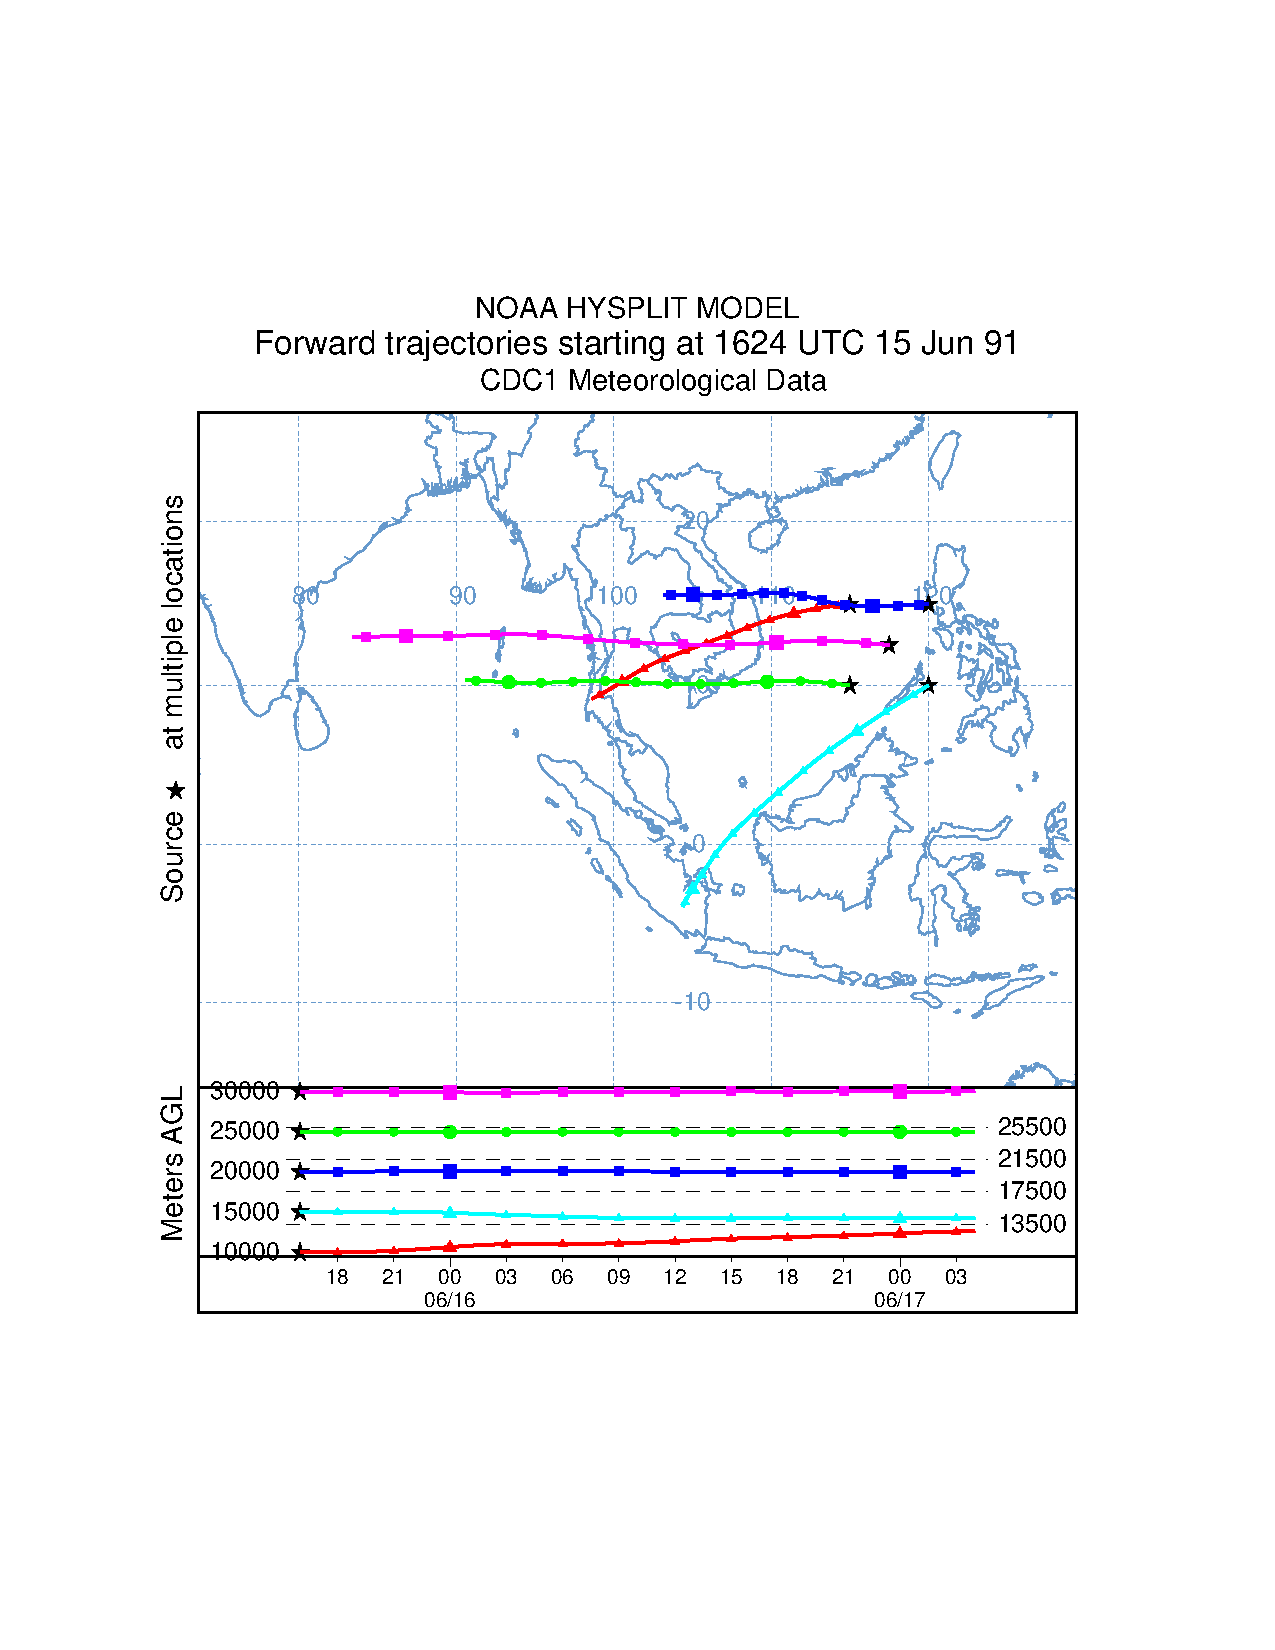
\includegraphics[width=0.99 \textwidth]{Figures/trajplot_test3_10_30K_ok}
\end{minipage}%
\caption{Trajectories of particles starting from different heights indicating the wind directions of different evaluations. The rajectories are choosen to start at points that were on the perimeter of the umbrella cloud in $x$, $y$ and $z$, and in its center, right before it became affected by the wind to give an idea of the maximum possible spread of the trajectories from that initial condition.}
\label{fig:hysplit-1624-utc}
\end{figure}

\begin{figure}[!htb]
\centering
\includegraphics[width=1.0\textwidth]{Figures/particle_distribution_vertical_compare}
\caption{First row, comparison of particle distribution of initial ash cloud in vertical direction. (a) is corresponding to the initial ash cloud obtained from Plume-SPH output. (b) is (a) truncated by a elevation threshold of 15 km. (c) is for vertical ash distribution based on Poisson distribution (Eq. (\ref{eq:Poisson-plume-shape})) with $H_{max}$ equals to 40 km. Another parameter, $H_{width}$ is 6662 m. (d) is corresponding to Suzuki distribution (Eq. (\ref{eq:Suzuki-plume-shape})) with $H_{max}$ equals to 40 km and $k$ equals to 4\citep{pfeiffer2005model}. The second row, Suzuki distribution with $H_{max}$ equals to 40 km but different values for $k$. The $x$ axis is the percentage of particle numbers for Plume-SPH and Poisson. For Suzuki the $x$ axis is the mass percentage of erupted material.}
\label{fig:Particle-distribution-Plume-SPH-vs-semiempirical}
\end{figure}

\begin{figure}[!htb]
\centering
\includegraphics[width=1.0\textwidth]{Figures/particle_distribution_vertical_calibration}
\caption{Initial particle distribution in vertical direction based on Poisson plume shape  (Eq. (\ref{eq:Poisson-plume-shape})). The first row varies plume heights. (a) to (d) are corresponding to plume height of 10 km, 20 km, 30 km, 35 km. Another parameter, $H_{width}$ is 6662 m for all four figures in the first row. The second row varies ``vertical spread", $H_{width}$. (e) to (g) are corresponding to vertical spread of 3 km, 5 km and 10 km. The plume height, $H_{max}$ is set to 40 km for all three figures. The $x$ axis is the percentage of particle numbers. See Fig. \ref{fig:Particle-distribution-Plume-SPH-vs-semiempirical} for vertical ash distribution of Plume-SPH output.}
\label{fig:Particle-distribution-Plume-calibrate-semiempirical}
\end{figure}

\begin{figure}[!htb]
\centering
\includegraphics[width=0.50 \textwidth]{Figures/radius-Plume-SPH-And-Assumed}
\caption{Comparison between radius of initial ash clouds created by 3D plume model (Plume-SPH) and assumed initial ash cloud shape (Eq. \ref{eq:horizontal-particle-distribution}) in Puff. The plume shape expression used in Puff defines an inverted cone whose actual shape changes when ``horizontal spread" takes different values. $R=$ 25 km is corresponding to ``horizontal spread" equals to 50 km. $R=$ 50 km is corresponding to ``horizontal spread" equals to 100 km}
\label{fig:radius-comparison}
\end{figure}

\begin{figure}[!htb]
\centering
\includegraphics[width=1.0\textwidth]{Figures/particle_horizontal_distribution}
\caption{Horizontal distribution of ash particles (tracers) on a cross section of initial ash cloud. Puff assumes a randomly uniform distribution of ash particles within a circle, as shown by blue dots in (f). All other figures show the ash particle distribution of initial ash clouds created by Plume-SPH at different elevations.}
\label{fig:initial-cloud-horizontal}
\end{figure}

\begin{figure}[!htb]
\centering
\includegraphics[width=0.80 \textwidth]{Figures/discussion}
\caption{Ash transport simulated by Puff using different initial ash clouds created according the empirical expressions using different input parameters. All images are corresponding to 55 hours after eruption (UT 199106171141). More details are in the table below}
	 \begin{tabular}{l|rrrr|rrr|rr}
	 \hline
            Parameter& \multicolumn{4}{c|}{$H_{max}$}& \multicolumn{3}{c|}{$H_{width}$} &  \multicolumn{2}{c}{$r_{max}$}\\
	 \cline{2-5}
	 \hline 
	 Value &10 km &20 km &30 km &35 km &3 km & 5km & 10 km &50 km&600 km \\
	 Plot& (a) & (b) & (c) &  (d) & (e) & (f) &  (g) & (h) &(i) \\
            FMS& 0.055 & 0.121& 0.142 &  0.227 & 0& 0.039 & 0.085 & 0.073 & 0.074  \\
	 \hline
	 \end{tabular}
\label{fig:discussion-initial-ash}
\end{figure}
T
\begin{figure}[!htb]
\centering
\includegraphics[width=0.99 \textwidth]{Figures/duration_cutoff}
\caption{Sensitivity of Puff simulation with respect to eruption durations and initial ash cloud cutoff heights (elevation threshold). For different eruption durations, the starting and ending time for each case is in Table \ref{tab:Pinatubo-eruption-duration}. The contours correspond to ash concentration at 72 hours after eruption. Details are in the table below.}
	 \begin{tabular}{l|rrr|rr}
	 \hline
            Parameter& \multicolumn{3}{c|}{Eruption Duration}& \multicolumn{2}{c}{Elevation Threshold}\\
	 \cline{2-4}
	 \hline 
	 Value &4.9 hour & 9 hour & 11.1 hour &1500 m &15 km \\
	 Plot& (a) & (b) & (c) &  (d) & (e) \\
	 \hline
	 \end{tabular}
\label{fig:Puff-sensitivity-duration-cutoff} 
\end{figure}

\begin{table}[htp]
	\centering
\caption{List of eruption condition and material properties for plume simulation}		
	 \begin{tabular}{lrr}
	 \hline
	 Parameters & Units & Plume \\
	 \hline
	 Vent Velocity & $\mathrm{m}\cdot \mathrm{s}^{-1}$ & 275 \\
	 Vent Gas Mass Fraction & & 0.05 \\
	 Vent Temperature & K & 1053 \\
	 Vent Height & m & 1500 \\
	 Mass Discharge Rate & $\mathrm{kg}\cdot \mathrm{s}^{-1}$ & $1.5 \times 10^9$\\
	 	Specific Heat of Gas at Constant Volume & $\mathrm{J} \cdot \mathrm{kg}^{-1}\cdot \mathrm{K}^{-1}$ & 717 \\
	 	Specific Heat of Air at Constant Volume &  $\mathrm{J} \cdot \mathrm{kg}^{-1}\cdot \mathrm{K}^{-1}$ & 1340 \\
	 	Specific Heat of Solid & $\mathrm{J} \cdot \mathrm{kg}^{-1}\cdot \mathrm{K}^{-1}$ & 1100 \\
	 	Specific Heat of Gas at Constant Pressure & $\mathrm{J} \cdot \mathrm{kg}^{-1}\cdot \mathrm{K}^{-1}$ & 1000 \\
	 	Specific Heat of Air at Constant Pressure & $\mathrm{J} \cdot \mathrm{kg}^{-1}\cdot \mathrm{K}^{-1}$ & 1810 \\
	 	Density of Air at Vent Height & $\mathrm{kg} \cdot \mathrm{m}^{-3}$ & 1.104 \\
	 Pressure at Vent Height & $\mathrm{Pa}$ & 84363.4 \\
	 \hline
	 \end{tabular}
	 \label{tab:input_parameters_plume_simulation}
\end{table}

\begin{table}[htp]
\centering
\caption{Parameters used in VATD simulation of the climactic phase of Pinatubo eruption on June 15 1991. The first six parameters are used by semiempirical expression to create an initial ash cloud. When creating an initial condition based on the Plume-SPH model, these parameters are extracted from output of Plume-SPH model.}
	 \begin{tabular}{lrrr}
	 \hline
	 Parameters & Unit & Semiempirical & Plume-SPH \\
	 \hline
	 Plume Height ($H_{max}$) & km & 40 & - \\ 
	 Horizontal Spread ($r_{max}$) & km & 103.808 & -\\
	 Vertical Spread ($H_{width}$) & km & 6.662 & - \\
	 Plume Shape & - & Poisson & - \\
	 Total Ash Particles & - & 1768500 & 1768500 \\
	 Elevation Threshold & m & - & 15000 \\
	 Horizontal Diffusivity & $\mathrm{m}^2/\mathrm{s}$ &10000 & 10000\\
	 Vertical Diffusivity & $\mathrm{m}^2/\mathrm{s}$ & 10 & 10 \\
	 Grain Size Distribution & - & Gaussian & Gaussian \\
	 Mean of Grain Size (Radius) & mm & $3.5 \times 10 ^-2$ & $3.5 \times 10 ^-2$ \\
	 Standard Deviation of Grain Size & - & 1.0 & 1.0 \\
	 	Start Time & UT & 0441 & 0441 \\
	 End time & UT & 1341 & 1341 \\
	 Simulation Duration & hour & 72 & 72 \\
	 \hline
	 \end{tabular}
	 \label{tab:input_parameter_Puff_simulation}
\end{table}

\begin{table}[htp]
\centering
\caption{The starting and ending time (UT) for simulating the climactic phase of Pinatubo eruption on June 15 1991. Observed plume height \citep{holasek1996satellite} at different time are also listed in the table.}		
	 \begin{tabular}{p{35mm}p{20mm}p{20mm}p{20mm}p{20mm}}
	 \hline
Eruption Duration & 4.9 hours & 9 hours & 10 hours & 11.1 hours \\
	 \hline
	 Start Time & 0441 & 0441 & 0441 & 0334 \\
	 Height at Start Time & 37.5 km & 37.5 km & 37.5 km & 24.5 km \\
	
	 End Time & 0934 & 1341 & 1441 & 1441 \\
	 Height at End Time & 35 km & 26.5 km & 22.5 & 22.5 km \\
	 \hline
	 \end{tabular}
	 \label{tab:Pinatubo-eruption-duration}
\end{table}
\end{document}
